% Disable copyright notice in the bottom right corner of the document since this document 
%   is not the intellectual property of ASME
% Technically, ASME standards say all text must be in black when papers are submitted for 
%   publication, but this isn't going to be submitted so we can enable colorlinks to get 
%   links to show up as blue.
\documentclass[nofoot,pdf-a,balance,colorlinks,upint,subscriptcorrection,varvw,mathalfa=cal=boondoxo]{asmeconf}
\special{papersize=8.5in,11in}

% % enable use of multiple files 
% % https://www.overleaf.com/learn/latex/Multi-file_LaTeX_projects
% % \usepackage{subfiles}
% \usepackage[subpreambles=true]{standalone}
% \usepackage{import}

\usepackage{amsmath}
% prevent Bbbk from being overdefined by amsmath and newtxmath (from asmeconf.cls)
\let\Bbbk\relax
\usepackage{mathtools}
\usepackage{amssymb}
\usepackage{xfrac}
% \usepackage[margin=1.00in]{geometry}
% \usepackage{tabto}
\usepackage{tikz}
\usepackage{pgfplots}
\usepackage[thinc]{esdiff}
\usepackage{float}
\usepackage{graphicx}

% enable use of multiple files 
% https://www.overleaf.com/learn/latex/Multi-file_LaTeX_projects
\usepackage{subfiles}

% PDF meta data
\hypersetup{
	pdfauthor={Lucas S. Johnston, Brendan Moskalik},
    pdftitle={Solution for the Dynamics Piston Project},
	pdfkeywords={Dynamics, Piston, Pins, Reactive forces, Project},
	pdfsubject = {Solution for the Dynamics Piston Project},
}

\begin{document}
    \ConfName{Proceedings of the Dynamics 2024 Local Mechanical Engineering Class and Exposition}
    \ConfDate{Spring, 2024} % update 
    \ConfCity{Spokane, WA}
    % let paper 0001 refer to our previous paper we submitted
    \PaperNo{ENSC2024-0002}

    \title{Piston Project}
    \SetAuthors{Lucas S. Johnston\affil{1}\JointFirstAuthor, Brendan Moskalik\affil{1}\JointFirstAuthor}
	\SetAffiliation{1}{Gonzaga University, Spokane, WA}

    \maketitle

    \begin{abstract}
        This paper is an analysis of the forces acting in pins within a crank-piston combination given a variety of cases. It analyzes the time-evolution of the system to derive an equation relating the forces in the pins to time in general, and applies specific conditions to create graphical representations of these forces for use in design. It is intended to be accompanied by a related MATLAB script \texttt{piston_script.m}, which is provided via a link to a git repository in the Appendix \ref{appendix:sources}.
    \end{abstract}

    \begin{nomenclature}
        \EntryHeading{Forces}
        \entry{$A$}{Shear force at A [N]}
        \entry{$P$}{Shear force at P [N]}

        \EntryHeading{Constant Parameters}
        \entry{$\omega$}{Angular velocity of the crank [rad s$^{-1}$]}
        \entry{$H$}{Offset distance between piston path and crank axis [m]}
        \entry{$L$}{Length of connecting rod [m]}
        \entry{$R$}{Distance from crank axis to point A [m]}
        \entry{$\theta_0$}{Initial angle of crank [rad]}
        \entry{$g$}{Gravitational acceleration [m s$^{-2}$]}\newline
       
        \EntryHeading{Time Evolution Parameters}
        \entry{$t$}{Time [s]}
        \entry{$\omega_{\textrm{AP}}$}{Angular velocity of the rod AP [rad s$^{-1}$]}
        \entry{$\alpha_{\textrm{AP}}$}{Angular acceleration of the rod AP [rad s$^{-2}$]}
        \entry{$m$}{Mass [kg]}
        \entry{$\vec{r}$}{Position [m]}
        \entry{$\vec{v}$}{Translational velocity [m s$^{-1}$]}
        \entry{$\vec{a}$}{Translational acceleration [m s$^{-2}$]}
        \entry{$\theta$}{Angle of crank with horizontal [rad]}\newline

        % TODO -- find a way to incorporate subscripts that 
        \EntryHeading{Superscripts and subscripts}
        \entry{x}{Horizontal component}
        \entry{y}{Vertical component}
        \entry{O}{Point O value}
        \entry{A}{Point A value}
        \entry{P}{Point P value}
        \entry{p}{Piston value}
        \entry{c}{Connecting rod AP value}
        \entry{$AP$}{Connecting rod AP value}
        
    \end{nomenclature}

    \section{Problem Statement}

    We are given a slider-crank piston setup explicitly parameterized by $L$, $R$, $H$, $\omega$, and $\theta$. With the exception of $\theta$, these parameters are all constant with respect to time. Information on these constant parameters can be found in Appendix \ref{appendix:cases}. The mass of the connecting rod and the piston ($m_{\textrm{c}}$ and $m_{\textrm{p}}$ respectively) are known, as is $R$. The rod is a cylinder with uniformly distributed mass per unit length.
    
    \begin{figure}[H]
        \centering
    	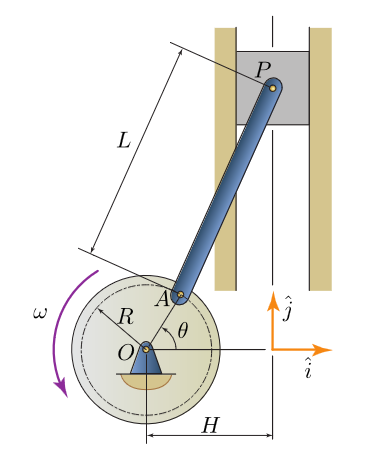
\includegraphics[scale=0.45]{problem_diagram.png}
    	\caption{Offset slider-crank piston, as given}\label{fig:diagram}
    \end{figure}

    \begin{table}[H]
        \caption[Table]{Case-Independent Known Values}\label{tab:given}
        \centering{
            \begin{tabular}{llr}
            \toprule
            Value & Value  & Units \\
            \midrule
                $R$ & 0.075 & m \\
                $m_{\textrm{c}}$ & 0.3 & kg \\
                $m_{\textrm{p}}$ & 0.4 & kg \\
            \bottomrule
            \end{tabular}
        }
    \end{table}

    The crank rotates about a fixed axis O. The piston is constrained to move up and down in the direction of the $\hat{\jmath}$ elementary vector as drawn. All motion is constrained to the plane spanned by $\hat{\imath}$ and $\hat{\jmath}$.


    \section{Solution Derivation}

    Let's solve the generic solution, and then apply specific cases to it once we've obtained useful formulas. We are interested in how the system evolves as $\theta$ changes. The rate of change of $\theta$, $\omega$ is given as a known constant. Therefore, we can parameterize $\theta$ as follows.
    \begin{equation} 
        \theta = \omega t + \theta_0
    \end{equation}
    Here, $\omega$ must be in radians per second (and therefore has to be converted from the as-given speeds given in rpm). $\theta_0$ refers to the initial condition of $\theta$ when $t = 0$ seconds.

    We are interested in finding the angular and translational acceleration of G, the center of gravity of the connecting rod for use in solving reactive forces at the pins A and B.


    This allows us to construct the position vector of A. Let the origin be set at fixed point O.

    \begin{equation} 
        \vec{r}_{\textrm{A}} = R\cdot\left(\cos{\left(\theta\right)}\hat{\imath} + \sin{\left(\theta\right)}\hat{\jmath}\right)
    \end{equation}


    The point A is constained to circular motion with a constant radius about the crank with a constant angular velocity.

    \begin{equation} 
        \vec{v}_{\textrm{A}} = \vec{0} + \omega\hat{k}\times\vec{r}_{\textrm{A}} = \omega\cdot\vec{r}_{\textrm{A}}
    \end{equation}


    Here $\hat{k}$ is a unit vector that, together with $\hat{\imath}$ and $\hat{\jmath}$, spans $\mathbb{R}^3$. This allows the cross product to be defined. $\hat{k}$ is normal to both $\hat{\imath}$ and $\hat{\j}$, and form the basis for a Cartesian representation of vectors in three-space in a Right Handed coordinate system. The angular velocity $\omega$ is given to us in a direction pointing in the $+\hat{k}$ direction.

    Let's now find the angular velocity of the rod to determine its acceleration. Since the rod has a constant length $L$, we can apply the following.

    \begin{equation} 
        % \, is a small space
        \vec{v}_{\,\textrm{P}} = \vec{v}_{\textrm{A}} + \omega_{\textrm{AP}}\hat{k}\times \vec{r}_{\,\sfrac{\textrm{P}}{\textrm{A}}}
    \end{equation}

    To find $\vec{r}_{\,\sfrac{\textrm{P}}{\textrm{A}}}$, we can build P's position from O.

    \begin{equation}
        \vec{r}_{\,\sfrac{\textrm{P}}{\textrm{A}}} + \vec{r}_{\textrm{A}} = \vec{r}_{\,\textrm{P}}
    \end{equation}
    \begin{equation}
        \hat{i}\cdot \left(\vec{r}_{\,\sfrac{\textrm{P}}{\textrm{A}}} + \vec{r}_{\textrm{A}}\right) = \hat{i} \cdot \left(\vec{r}_{\,\textrm{P}}\right)
    \end{equation}
    \begin{equation}
        \hat{i}\cdot \vec{r}_{\,\sfrac{\textrm{P}}{\textrm{A}}} = \hat{\imath} \cdot \vec{r}_{\,\textrm{P}} - \hat{\imath} \cdot\vec{r}_{\textrm{A}} 
    \end{equation}
    \begin{equation}
        \hat{i}\cdot \vec{r}_{\,\sfrac{\textrm{P}}{\textrm{A}}} = H - R\cdot\cos{\left(\theta\right)}
    \end{equation}

    Applying the constraint that the distance from point A to point P is $L$, we get the following.

    \begin{equation} 
        L^2 = \left(\vec{r}_{\,\sfrac{\textrm{P}}{\textrm{A}}} \cdot\hat{\imath} \right)^2+ \left(\vec{r}_{\,\sfrac{\textrm{P}}{\textrm{A}}} \cdot\hat{\jmath}\right)^2
    \end{equation}

    Since the vertical component of $\vec{r}_{\,\sfrac{\textrm{P}}{\textrm{A}}}$ is positive as drawn in Fig \ref{fig:diagram}, we use the positive root.
    \begin{equation} 
        \vec{r}_{\,\sfrac{\textrm{P}}{\textrm{A}}} \cdot\hat{\jmath} = \sqrt{L^2 - \left(\vec{r}_{\,\sfrac{\textrm{P}}{\textrm{A}}} \cdot\hat{\imath} \right)^2}
    \end{equation}
    \begin{equation} 
        \vec{r}_{\,\sfrac{\textrm{P}}{\textrm{A}}} \cdot\hat{\jmath} = \sqrt{L^2 - \left(H - R\cdot\cos{\left(\theta\right)}\right)^2}
    \end{equation}

    $\vec{r}_{\,\sfrac{\textrm{P}}{\textrm{A}}}$ is now well-defined.

    \begin{equation} 
        \vec{r}_{\,\sfrac{\textrm{P}}{\textrm{A}}} = \left(H - R\cdot\cos{\left(\theta\right)}\right)\hat{\imath} + \left(\sqrt{L^2 - \left(H - R\cdot\cos{\left(\theta\right)}\right)^2}\right)\hat{\jmath}
    \end{equation}
    
    We can now use the fact that $\vec{v}_{\,\textrm{P}}$ is constrained to purely vertical movement. Let $v_{\,\textrm{P}} = \vec{v}_{\,\textrm{P}} \cdot \hat{\jmath}$. 

    \begin{equation} 
        v_{\,\textrm{P}}\hat{\jmath} = \vec{v}_{\textrm{A}} + \omega_{\textrm{AP}}\hat{k}\times \vec{r}_{\,\sfrac{\textrm{P}}{\textrm{A}}}
    \end{equation}

    Every variable in the above expression is a `known' quantity expressible purely in terms of constant parameters and time, with the exception of $v_{\,\textrm{P}}$ and $\omega_{\textrm{AP}}$. These scalar quantities are, in essence, two degrees of freedom now being constrained within a vector equation. This vector equation can be broken into two linearly dependent equations, which suggest $v_{\,\textrm{P}}$ and $\omega_{\textrm{AP}}$ are both well-defined. It is left as an exercise to the reader to prove the following.%We can manipulate this expression to pull known quantities off to one side of the equation, and factor a matrix in Mat($\mathbb{R}$)$^{2\times 2}$. Since we will be dealing with matrices, it is more illustrative to write vectors as column vectors.
    % TODO -- resume work here

    \subfile{autogen_vel}



    Let $A$ represent the magnitude of the forces on the pin at A and let $P$ represent the magnitude of the forces on the pin at P. We can derive the following expressions. Using the property of the magnitude of vectors, we can derive the following in terms of equations defined in Appendix \ref{appendix:definitions}.
    \begin{equation}
        A = \sqrt{A_{\textrm{x}}^2 + A_{\textrm{y}}^2}
    \end{equation}
    Here, $A_{\textrm{x}}$ is defined in Eq. \eqref{A:x} and $A_{\textrm{y}}$ is defined in Eq. \eqref{A:y}.
    \begin{equation}
        P = \sqrt{P_{\textrm{x}}^2 + P_{\textrm{y}^2}}
    \end{equation}
    $P_{\textrm{x}}$ is defined in Eq. \eqref{P:x} and $P_{\textrm{y}}$ is defined in Eq. \eqref{P:y}.

    \appendix
    \section{Cases}\label{appendix:cases}
	  \begin{table}[H]
        \caption[Table]{Cases to consider (Given)}\label{tab:givenCases}
        \centering{
            \begin{tabular}{llr}
            \toprule
            Case & L/R  & H/R \\
            \midrule
                1 & \sfrac{3}{2} & 0 \\
                2 & \sfrac{8}{3} & \sfrac{1}{3} \\
                3 & 4 & \sfrac{5}{3} \\
            \bottomrule
            \end{tabular}
        }
    \end{table}

	Since we know the radius of all these cases to be 0.075 m we can compute values for L and H. Plugging those in:
\begin{table}[H]
        \caption[Table]{Cases to consider (Absolute)}\label{tab:absCases}
        \centering{
            \begin{tabular}{llr}
            \toprule
            Case & L (m)  & H (m) \\
            \midrule
                1 & 0.1124 & 0 \\
                2 & 0.2 & 0.025 \\
                3 & 0.3 & 0.125 \\
            \bottomrule
            \end{tabular}
        }
    \end{table}


    \subfile{autogen_fn_def}

    \section{Sources}\label{appendix:sources} 

    This document was written with \LaTeX\ and is designed to be compilled by a valid \LaTeX\ engine such as \texttt{pdflatex}. The git repository used to generate this document can be found online on GitHub at \href{https://github.com/A-Person7/dynamics_piston_project}{https://github.com/A-Person7/dynamics_piston_project}. MATLAB's symbolic toolbox was used to solve a lot of the linear algebra shown throughout this document, as well as to generate equations. These were implemented in the MATLAB script file \texttt{piston_script.m}. Compilation instructions for the final document are provided in the plain-text file \texttt{README}.

    \end{document}
